\documentclass[a4paper,12pt]{article}
\usepackage[utf8]{inputenc}
\usepackage{amsmath, amssymb, amsthm} % For math symbols and environments
\usepackage{graphicx} % For including images
\usepackage{hyperref} % For hyperlinks
\usepackage{fancyhdr} % For header and footer
\usepackage{geometry} % For adjusting page dimensions
\usepackage{cite} % For handling references
\geometry{margin=1in}

% Header and footer
\pagestyle{fancy}
\fancyhf{}
\fancyhead[L]{Sravanth Chowdary Potluri}
\fancyhead[C]{ML On Graphs HW1}
\fancyhead[R]{\thepage}
\fancyfoot[L]{CS6501 - 016}
\fancyfoot[R]{\today}

% Title Page
\title{Machine Learning On Graphs HW1}
\author{Sravanth Chowdary Potluri \\ und5uv \\ CS6501 - 016}
\date{\today}

\begin{document}

\maketitle

\section{Problem 1: Adjacency Matrix (25 pts)}

Consider an undirected graph \( G \) with adjacency matrix \( A \). Denote \( A_i \) as the \( i \)th row and \( A_{ij} \) as the element at row \( i \) and column \( j \).

\begin{enumerate}
    \item How can we compute the number of common neighbors between vertex \( i \) and vertex \( j \)? (3 pts)
    \item The number of triangles in the graph \( G \)? (5 pts)
    \item The number of walks of length \( k \)? (5 pts)
    \item What is challenging about computing the number of paths using the adjacency matrix? (6 pts)
    \item How can we determine if the graph is connected using the adjacency matrix? (6 pts)
\end{enumerate}

\section*{Solution 1}

Consider an undirected graph \( G \) with adjacency matrix \( A \), where \( A_i \) denotes the \( i \)th row of \( A \) and \( A_{ij} \) the \((i,j)\)th entry. We answer the questions as follows:

\begin{enumerate}
    \item \textbf{Number of Common Neighbors:} \\
    The number of common neighbors between vertices \( i \) and \( j \) is given by the dot product of the \( i \)th and \( j \)th rows of \( A \). In other words,
    \[
    \text{Number of common neighbors} = \sum_{k} A_{ik} A_{jk} = (A^2)_{ij}.
    \]
    Here, \( (A^2)_{ij} \) counts exactly how many vertices \( k \) are adjacent to both \( i \) and \( j \).

    \item \textbf{Number of Triangles:} \\
    A triangle in \( G \) corresponds to a cycle of length 3. It is known that the \((i,i)\)th entry of \( A^3 \), that is, \( (A^3)_{ii} \), counts the number of 2-walks (of length 3) starting and ending at vertex \( i \). Summing over all vertices gives \( \text{tr}(A^3) \), but notice that in an undirected graph each triangle is counted 6 times (each triangle has 3 vertices and it can be traversed in 2 directions). Hence, the total number of triangles is
    \[
    \text{Number of triangles} = \frac{1}{6}\,\mathrm{tr}(A^3).
    \]

    \item \textbf{Number of Walks of Length \( k \):} \\
    The \((i,j)\)th entry of \( A^k \) gives the number of walks of length \( k \) from vertex \( i \) to vertex \( j \). That is,
    \[
    \text{Number of walks of length } k \text{ from } i \text{ to } j = (A^k)_{ij}.
    \]

    \item \textbf{Challenges in Computing the Number of Paths:} \\
    A \emph{walk} is a sequence of vertices (and edges) where vertices (and edges) may be repeated, and as we have seen, the powers \( A^k \) count walks. However, a \emph{path} is a walk in which no vertex is repeated. The challenge in computing the number of paths using the adjacency matrix is that the matrix powers do not distinguish between walks that revisit vertices and those that do not. In order to count only simple paths (with no repetitions), one would have to somehow exclude from \( A^k \) all the walks that are not paths. This typically requires complicated combinatorial adjustments (often involving the principle of inclusion–exclusion) and, in many cases, leads to computational problems that are NP–hard.

    \item \textbf{Determining if the Graph is Connected:} \\
    A graph is connected if there is a walk between every pair of vertices. One way to check for connectivity is to verify that for every pair \( (i,j) \) there exists some \( k \) (with \( 1 \le k \le n-1 \), where \( n \) is the number of vertices) such that
    \[
    (A^k)_{ij} > 0.
    \]
    Equivalently, one can form the Boolean matrix
    \[
    R = I \vee A \vee A^2 \vee \cdots \vee A^{n-1},
    \]
    where \( \vee \) denotes the Boolean OR operation (i.e., an entry is 1 if at least one corresponding entry in the summands is nonzero). If every entry of \( R \) is 1, then every vertex is reachable from every other vertex and the graph is connected.

\end{enumerate}

% \section*{Solution 2}

% \begin{enumerate}
%     \item \textbf{Number of common neighbors between vertex \(i\) and vertex \(j\) (3 pts)}\\[6pt]
%     The number of common neighbors is given by the dot product of the \(i\)th and \(j\)th rows of the adjacency matrix \(A\). In other words,
%     \[
%     \text{CommonNeighbors}(i,j) \;=\; \sum_{\ell} A_{i,\ell} \, A_{j,\ell}.
%     \]
%     This sum effectively counts how many vertices \(\ell\) are adjacent to both \(i\) and \(j\).

%     \item \textbf{Number of triangles in the graph \(G\) (5 pts)}\\[6pt]
%     For an undirected graph, the total number of triangles can be obtained from the trace of \(A^3\).  Specifically, each triangle is counted 6 times in \(\mathrm{trace}(A^3)\), so
%     \[
%     \text{Number of triangles} \;=\; \frac{\mathrm{trace}(A^3)}{6}.
%     \]
%     Here, \(\mathrm{trace}(A^3)\) is the sum of the diagonal entries of \(A^3\).

%     \item \textbf{Number of walks of length \(k\) (5 pts)}\\[6pt]
%     If we let \(A^k\) denote the \(k\)-th power of the adjacency matrix \(A\), then the \((i,j)\)-entry of \(A^k\) equals the number of distinct walks of length \(k\) from vertex \(i\) to vertex \(j\).  Thus:
%     \[
%     (A^k)_{ij} \;=\; \text{number of walks of length \(k\) from \(i\) to \(j\).}
%     \]
%     If one wants the total number of walks of length \(k\) in the entire graph (over all start/end vertices), one can sum all the entries of \(A^k\).

%     \item \textbf{What is challenging about computing the number of paths using the adjacency matrix? (6 pts)}\\[6pt]
%     A \emph{walk} may repeat vertices and edges, whereas a \emph{simple path} may not.  The matrix powers \(A^k\) count all walks, including those that revisit vertices.  To count only simple paths of length \(k\), one must exclude walks that loop back or revisit vertices, and there is no straightforward matrix-based formula for doing so.  Consequently, directly using matrix powers to count simple paths quickly becomes complicated, because one must track and avoid repeated vertices.

%     \item \textbf{How to determine if the graph is connected using the adjacency matrix? (6 pts)}\\[6pt]
%     One matrix-based criterion for connectedness is the following: an undirected graph \(G\) on \(n\) vertices is connected if and only if, for every pair of vertices \(i\) and \(j\), there exists some integer \(k \le n-1\) such that \((A^k)_{ij} > 0\).  Equivalently, if we define 
%     \[
%     S \;=\; A + A^2 + \cdots + A^{n-1},
%     \]
%     then \(G\) is connected if and only if \(S_{ij} > 0\) for every \(i,j\).  Intuitively, this means there is a path (of some length at most \(n-1\)) connecting every pair of vertices.
% \end{enumerate}






\section{Problem 2: Shortest Paths and Minimum Spanning Tree (25 pts)}

\begin{enumerate}
    \item Detail why edges with negative weights are not desirable for computing shortest paths. (6 pts)
    \item Compute the shortest path between \( v_1 \) and \( v_9 \) using Dijkstra’s algorithm for the graph in Figure 1. Provide step-by-step details. (8 pts)
    \item Find a minimum spanning tree for the graph in Figure 1. Provide step-by-step details. (11 pts)
\end{enumerate}

\begin{figure}[h]
    \centering
    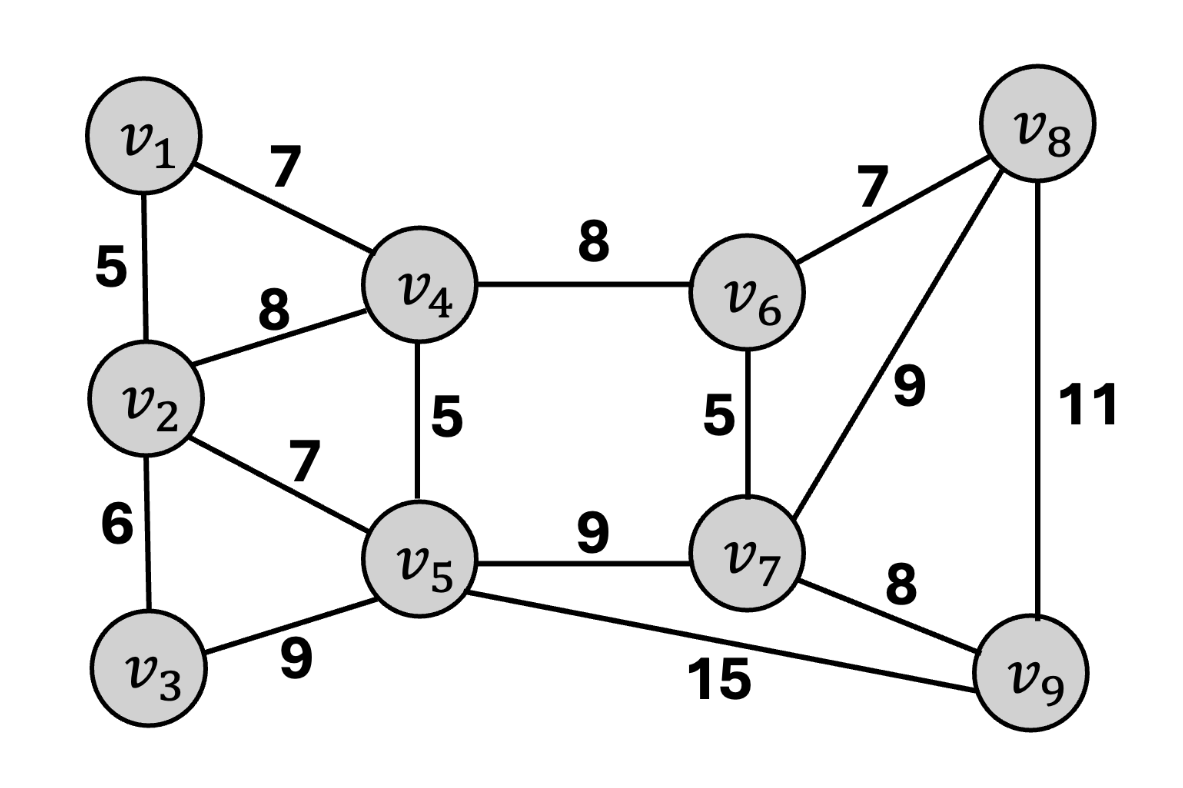
\includegraphics[width=0.6\textwidth]{p2.png} % Placeholder for Figure 1
    \caption{The input graph for Problem 2.}
    \label{fig:graph1}
\end{figure}

\section*{Solution}

\begin{enumerate}
    \item \textbf{Why edges with negative weights are not desirable for shortest paths (6 pts)}\\[6pt]
    Negative edge weights complicate shortest-path problems because many standard algorithms rely on the assumption that once a “best” partial path to a vertex has been found, it cannot be improved by later updates. More specifically:
    \begin{itemize}
        \item \textbf{Dijkstra's algorithm} requires nonnegative edge weights to ensure that when a vertex is “settled” (i.e., the shortest distance to it is found), there is no cheaper path discovered later.
        \item If a negative edge weight is allowed, repeatedly traversing a negative-weight cycle can reduce the total path length indefinitely, making the concept of a “shortest path” ill-defined.
        \item Even if there is no negative cycle, the presence of negative edges can invalidate the greedy steps used by Dijkstra’s algorithm, as an initially chosen “optimal” step might not remain optimal after accounting for the negative cost elsewhere.
    \end{itemize}
    In short, negative edge weights can violate the core assumptions that make many shortest-path algorithms both valid and efficient.
    
    \item \textbf{Shortest path between \(v_1\) and \(v_9\) using Dijkstra’s algorithm (8 pts)}\\[6pt]
    Consider the graph in the figure with vertices \(v_1, v_2, \ldots, v_9\). We label the edge weights as follows (assuming undirected edges):

    \[
    \begin{aligned}
    &(v_1, v_2) = 5,\quad (v_1, v_4) = 7,\\
    &(v_2, v_3) = 6,\quad (v_2, v_4) = 8,\quad (v_2, v_5) = 7,\\
    &(v_3, v_5) = 9,\\
    &(v_4, v_5) = 5,\quad (v_4, v_6) = 8,\\
    &(v_5, v_7) = 9,\quad (v_5, v_9) = 15,\\
    &(v_6, v_7) = 5,\quad (v_6, v_8) = 7,\\
    &(v_7, v_8) = 9,\quad (v_7, v_9) = 8,\\
    &(v_8, v_9) = 11.
    \end{aligned}
    \]

    
    \underline{Initialization}:
    \[
    \begin{aligned}
    \text{dist}(v_1) &= 0, \\
    \text{dist}(v_i) &= \infty \quad \text{for all } i = 2,3,\dots,9.
    \end{aligned}
    \]
    All vertices are unvisited; at each step, pick the unvisited vertex with the smallest tentative distance.

    \begin{enumerate}
        \item \textbf{Settle \(v_1\)}:
        \[
        \text{dist}(v_1) = 0.
        \]
        Update neighbors of \(v_1\):
        \[
        \text{dist}(v_2) \leftarrow 5, \quad \text{dist}(v_4) \leftarrow 7.
        \]
        
        \item \textbf{Settle \(v_2\)} (next smallest distance = 5):
        Update neighbors of \(v_2\):
        \[
        \text{dist}(v_3) \leftarrow 5 + 6 = 11, \quad
        \text{dist}(v_5) \leftarrow 5 + 7 = 12.
        \]
        \(\text{dist}(v_4)\) remains \(7\) (since \(5 + 8 = 13 > 7\)).
        
        \item \textbf{Settle \(v_4\)} (distance = 7):
        Neighbors: \((v_4, v_5) = 5\) and \((v_4, v_6) = 8\).
        \[
        \text{dist}(v_5) ? 7 + 5 = 12 \quad (\text{already } 12)\rightarrow \text{no change}.
        \]
        \[
        \text{dist}(v_6) \leftarrow 7 + 8 = 15.
        \]
        
        \item \textbf{Settle \(v_3\)} (distance = 11):
        Neighbor: \((v_3, v_5) = 9\).
        \[
        \text{dist}(v_5) ? 11 + 9 = 20 \quad (\text{already } 12)\rightarrow \text{no change}.
        \]
        
        \item \textbf{Settle \(v_5\)} (distance = 12):
        Neighbor: \((v_5, v_7) = 9\), \((v_5, v_9) = 15\) .
        \[
        \text{dist}(v_7) \leftarrow 12 + 9 = 21.
        \]
        \[
        \text{dist}(v_9) \leftarrow 12 + 15 = 27.
        \]

        
        \item \textbf{Settle \(v_6\)} (distance = 15):
        Neighbors: \((v_6, v_7) = 5\) and \((v_6, v_8) = 7\).
        \[
        \text{dist}(v_7) ? 15 + 5 = 20 < 21 \quad \rightarrow \text{dist}(v_7) = 20.
        \]
        \[
        \text{dist}(v_8) \leftarrow 15 + 7 = 22.
        \]
        
        \item \textbf{Settle \(v_7\)} (distance = 20):
        Neighbors: \((v_7, v_8) = 9\).
        \[
        \text{dist}(v_8) ? 20 + 9 = 29 \quad (\text{already }22)\rightarrow \text{no change}.
        \]
        
        \item \textbf{Settle \(v_8\)} (distance = 22):
        Neighbor: \((v_8, v_9) = 11\).
        \[
        \text{dist}(v_9) ? 22 + 11 = 33 \quad (\text{already } 27)\rightarrow \text{no change}.
        \]
        
        \item \textbf{Settle \(v_9\)} (distance = 27):
        No more updates since all others visited.
    \end{enumerate}

    Thus, \(\text{dist}(v_9) = 27\). Tracing predecessors back shows the path
    \[
    v_1 \;\to\; v_4 \;\to\; v_5 \;\to\; v_9 \;
    \]
    with total cost \(7 + 5 + 15 = 27.\)

    Alternatively, another path is.
    \[
    v_1 \;\to\; v_2 \;\to\; v_5 \;\to\; v_9 \;
    \]

    with total cost \(5 + 7 + 15 = 27.\)


    \item \textbf{Find a minimum spanning tree for the graph (11 pts)}\\[6pt]

    We use \textbf{Prim's algorithm} to find the MST of the graph with vertices \(v_1,\dots,v_9\) and edge weights:

    \[
    \begin{aligned}
    &(v_1, v_2) = 5,\quad (v_1, v_4) = 7,\\
    &(v_2, v_3) = 6,\quad (v_2, v_4) = 8,\quad (v_2, v_5) = 7,\\
    &(v_3, v_5) = 9,\\
    &(v_4, v_5) = 5,\quad (v_4, v_6) = 8,\\
    &(v_5, v_7) = 9,\quad (v_5, v_9) = 15,\\
    &(v_6, v_7) = 5,\quad (v_6, v_8) = 7,\\
    &(v_7, v_8) = 9,\quad (v_7, v_9) = 8,\\
    &(v_8, v_9) = 11.
    \end{aligned}
    \]

    \begin{enumerate}
    \item \textbf{Initialize:} Pick an arbitrary start vertex, say \(v_1\). The MST is initially empty, and the set of “in-tree” vertices is \(\{v_1\}\).

    \item \textbf{Step 1:} Among edges out of \(\{v_1\}\), the cheapest is \((v_1,v_2)\) with weight \(5\). Add it:
    \[
    \text{MST} = \{\,(v_1,v_2)\}, \quad \text{In-tree vertices} = \{v_1,v_2\}.
    \]

    \item \textbf{Step 2:} From \(\{v_1,v_2\}\) to outside, we have:
    \[
    (v_1,v_4)=7,\quad (v_2,v_3)=6,\quad (v_2,v_4)=8,\quad (v_2,v_5)=7.
    \]
    Cheapest is \((v_2,v_3)=6\). Add it:
    \[
    \text{MST} = \{\,(v_1,v_2),(v_2,v_3)\}, \quad \text{In-tree} = \{v_1,v_2,v_3\}.
    \]

    \item \textbf{Step 3:} Now from \(\{v_1,v_2,v_3\}\) to outside, the candidate edges are:
    \[
    (v_1,v_4)=7, \quad (v_2,v_4)=8, \quad (v_2,v_5)=7, \quad (v_3,v_5)=9.
    \]
    The cheapest are \((v_1,v_4)\) or \((v_2,v_5)\), both weight \(7\). Suppose we pick \((v_1,v_4)=7\). Then
    \[
    \text{MST} = \{\,(v_1,v_2),(v_2,v_3),(v_1,v_4)\}, \quad \text{In-tree} = \{v_1,v_2,v_3,v_4\}.
    \]

    \item \textbf{Step 4:} From \(\{v_1,v_2,v_3,v_4\}\) outwards, possible edges are:
    \[
    (v_2,v_5)=7, \quad (v_3,v_5)=9, \quad (v_4,v_5)=5, \quad (v_4,v_6)=8.
    \]
    The cheapest is \((v_4,v_5)=5\).  Add it:
    \[
    \text{MST} = \{\,(v_1,v_2),(v_2,v_3),(v_1,v_4),(v_4,v_5)\}, \quad \text{In-tree} = \{v_1,v_2,v_3,v_4,v_5\}.
    \]

    \item \textbf{Step 5:} Now \(\{v_6,v_7,v_8,v_9\}\) remain outside. The relevant edges from in-tree vertices are:
    \[
    (v_4,v_6)=8, \quad (v_5,v_7)=9, \quad (v_5,v_9)=15.
    \]
    The cheapest is \((v_4,v_6)=8\):
    \[
    \text{MST} = \{\,(v_1,v_2),(v_2,v_3),(v_1,v_4),(v_4,v_5),(v_4,v_6)\}, \quad \text{In-tree} = \{v_1,v_2,v_3,v_4,v_5,v_6\}.
    \]

    \item \textbf{Step 6:} Remaining outside are \(v_7,v_8,v_9\).  New edges from the in-tree to those outside are:
    \[
    (v_6,v_7)=5,\quad (v_6,v_8)=7,\quad (v_5,v_7)=9,\quad (v_5,v_9)=15.
    \]
    Cheapest is \((v_6,v_7)=5\).  Add it:
    \[
    \text{MST} 
    = \bigl\{\dots, (v_4,v_6),(v_6,v_7)\bigr\}, 
    \quad \text{In-tree} = \{v_1,v_2,v_3,v_4,v_5,v_6,v_7\}.
    \]

    \item \textbf{Step 7:} Outside are \(v_8,v_9\). From the in-tree to those outside are:
    \[
    (v_6,v_8)=7,\quad (v_7,v_8)=9,\quad (v_7,v_9)=8,\quad (v_5,v_9)=15.
    \]
    The cheapest is \((v_6,v_8)=7\).  Add it:
    \[
    \text{MST} = \{\dots,(v_6,v_8)\}, \quad \text{In-tree} = \{v_1,v_2,v_3,v_4,v_5,v_6,v_7,v_8\}.
    \]

    \item \textbf{Step 8:} Only \(v_9\) remains. Edges from the in-tree to \(v_9\) are:
    \[
    (v_5,v_9)=15,\quad (v_7,v_9)=8,\quad (v_8,v_9)=11.
    \]
    Cheapest is \((v_7,v_9)=8\).  Add it and we have a spanning tree on all 9 vertices:
    \[
    \text{MST} = \bigl\{
    (v_1,v_2), (v_2,v_3), (v_1,v_4), (v_4,v_5), (v_4,v_6), (v_6,v_7),
    (v_6,v_8), (v_7,v_9)
    \bigr\}.
    \]

    \item \textbf{Weights and Total:}\\[3pt]
    The MST edges and weights:
    \[
    5 + 6 + 7 + 5 + 8 + 5 + 7 + 8 \;=\; 51.
    \]
    Thus, the MST edges are:
    \[
    \{(v_1,v_2),(v_2,v_3),(v_1,v_4),(v_4,v_5),(v_4,v_6),(v_6,v_7),(v_6,v_8),(v_7,v_9)\},
    \]
    with total weight \(51\).
    \end{enumerate}
    \end{enumerate}




\section{Problem 3: PageRank (25 pts)}

\begin{enumerate}
    \item Calculate PageRank values for the graph in Figure 2 when:
    \begin{itemize}
        \item \( \alpha = 0.3, \beta = 0.5 \)
        \item \( \alpha = 0, \beta = 1 \)
    \end{itemize} (6 pts)
    \item Discuss the effects of different values of \( \alpha \) and \( \beta \) for this particular problem. (4 pts)
    \item Does \( \beta \) have any effect on the order of centralities? If for one value of \( \beta \), the centrality value of node \( v_i \) is greater than that of \( v_j \), is it possible to change \( \beta \) in a way such that \( v_j \)'s centrality becomes larger than that of \( v_i \)'s? (5 pts)
    \item In PageRank, what \( \alpha \) values can we select in order to guarantee that centrality values are calculated correctly, i.e., values do not diverge? (5 pts)
    \item Prove that the largest eigenvalue of matrix \( AD^{-1} \) is 1. (5 pts)
\end{enumerate}

\begin{figure}[h]
    \centering
    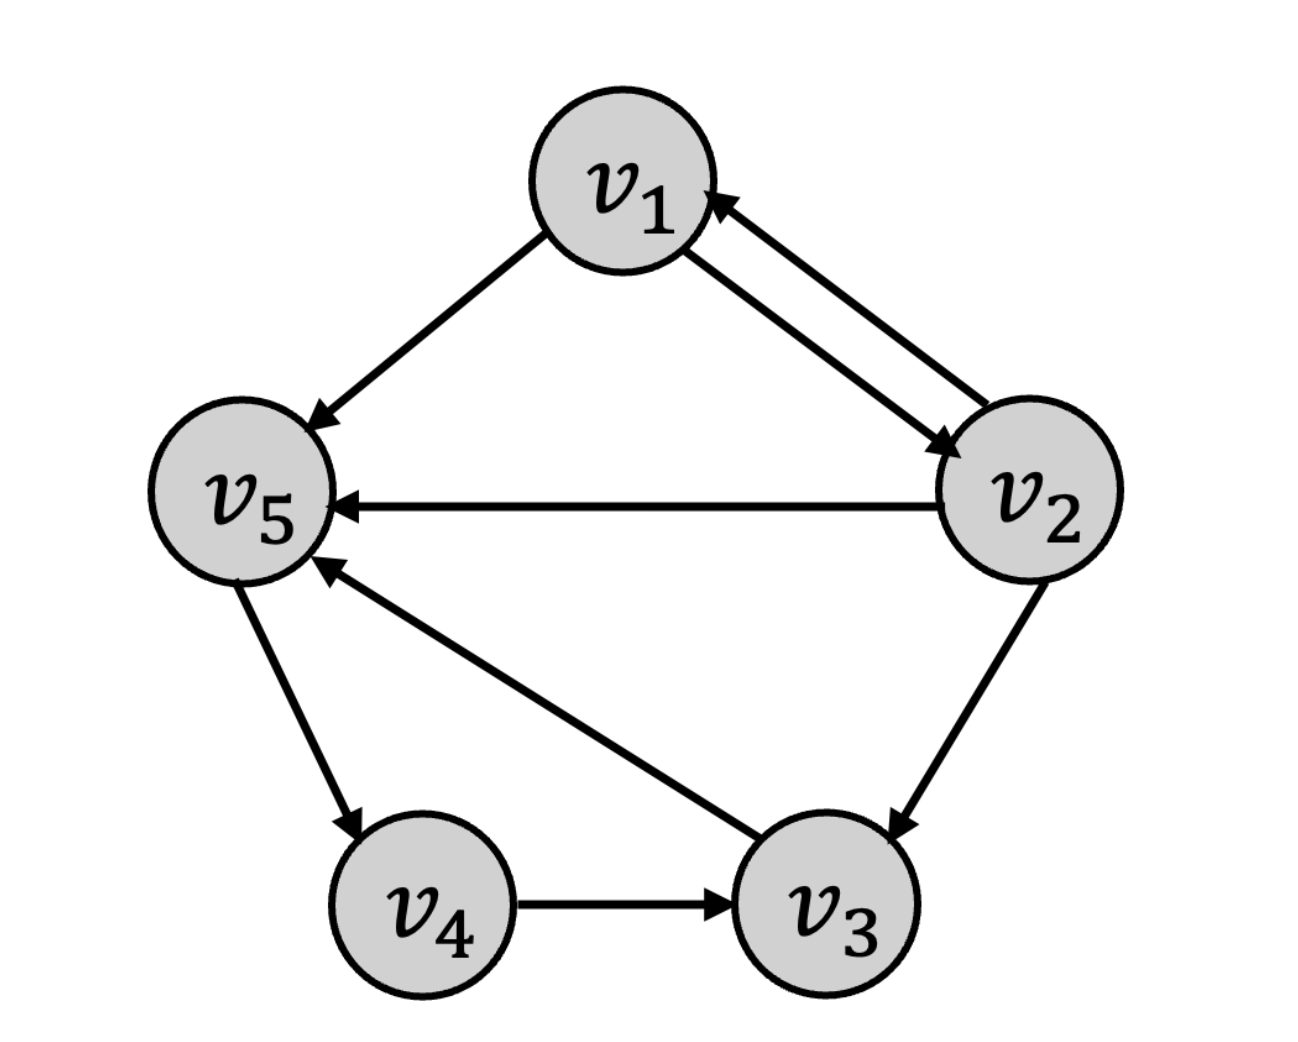
\includegraphics[width=0.6\textwidth]{p3.png} % Placeholder for Figure 2
    \caption{The input graph for Problem 3.}
    \label{fig:graph2}
\end{figure}

\section*{Solution}

We are given a directed graph on five vertices $v_1,\dots,v_5$ with edges
\[
\begin{aligned}
v_1 &\to \{v_2,\,v_5\}, && d_1^{\text{out}} = 2,\\
v_2 &\to \{v_3,\,v_5,\,v_1\}, && d_2^{\text{out}} = 3,\\
v_3 &\to \{v_5\}, && d_3^{\text{out}} = 1,\\
v_4 &\to \{v_3\}, && d_4^{\text{out}} = 1,\\
v_5 &\to \{v_4\}, && d_5^{\text{out}} = 1.
\end{aligned}
\]
We denote the adjacency matrix by $A = (a_{ij})$, where 
\[
a_{ij} \;=\;
\begin{cases}
1 & \text{if there is an edge }v_i\to v_j,\\
0 & \text{otherwise.}
\end{cases}
\]
The diagonal matrix of out-degrees is 
\[
D = \mathrm{diag}\bigl(d_1^{\mathrm{out}},\,d_2^{\mathrm{out}},\,\dots,\,d_5^{\mathrm{out}}\bigr)
= \mathrm{diag}(2,\,3,\,1,\,1,\,1).
\]
The PageRank--style centrality vector $\mathbf{C}_p$ can be written in matrix form as
\[
\mathbf{C}_p 
\;=\; 
\beta\;\bigl(I \;-\;\alpha\,A^\top\,D^{-1}\bigr)^{-1}\,\mathbf{1},
\]
where $\mathbf{1}$ is the all-ones vector $(1,1,\dots,1)^\top$, and $\alpha,\beta$ are parameters.

\medskip
Below, we carry out the steps:

\begin{enumerate}
% 1) ---------------------------------------------------------------------------------
\item \textbf{Calculate PageRank values for the graph in Figure 2 when:}
\begin{itemize}
\item $\alpha = 0.3,\;\beta = 0.5,$
\item $\alpha = 0,\;\beta = 1.$
\end{itemize}

\subsubsection*{(a) Constructing the necessary matrices}

\paragraph{Adjacency matrix $A$.}
Labeling vertices in the order $v_1,v_2,v_3,v_4,v_5$, the adjacency matrix is:
\[
A \;=\;
\begin{pmatrix}
0 & 1 & 0 & 0 & 1\\
1 & 0 & 1 & 0 & 1\\
0 & 0 & 0 & 0 & 1\\
0 & 0 & 1 & 0 & 0\\
0 & 0 & 0 & 1 & 0
\end{pmatrix},
\]
because:
\[
\begin{aligned}
&v_1 \to v_2,\,v_5 &&\implies \; a_{1,2}=1,\;a_{1,5}=1,\\
&v_2 \to v_3,\,v_5,\,v_1 &&\implies \; a_{2,3}=1,\;a_{2,5}=1,\;a_{2,1}=1,\\
&v_3 \to v_5 &&\implies \; a_{3,5}=1,\\
&v_4 \to v_3 &&\implies \; a_{4,3}=1,\\
&v_5 \to v_4 &&\implies \; a_{5,4}=1.
\end{aligned}
\]

\paragraph{Diagonal matrix of out-degrees $D$.}
\[
D 
\;=\;
\mathrm{diag}\bigl(2,3,1,1,1\bigr).
\]

\paragraph{Matrix $M = A^\top D^{-1}$.}
First note that $D^{-1} = \mathrm{diag}\!\bigl(\tfrac12,\tfrac13,1,1,1\bigr)$.
Then 
\[
A^\top \;=\;
\begin{pmatrix}
0 & 1 & 0 & 0 & 0\\
1 & 0 & 0 & 0 & 0\\
0 & 1 & 0 & 1 & 0\\
0 & 0 & 0 & 0 & 1\\
1 & 1 & 1 & 0 & 0
\end{pmatrix}.
\]
Hence each column $j$ of $A^\top$ is multiplied by $1/d_j^{\mathrm{out}}$, giving
\[
M \;=\; A^\top\,D^{-1} \;=\;
\begin{pmatrix}
0 & \tfrac{1}{3} & 0 & 0 & 0\\
\tfrac12 & 0 & 0 & 0 & 0\\
0 & \tfrac{1}{3} & 0 & 1 & 0\\
0 & 0 & 0 & 0 & 1\\
\tfrac12 & \tfrac{1}{3} & 1 & 0 & 0
\end{pmatrix}.
\]

\subsubsection*{(b) Case 1: \(\alpha = 0.3,\;\beta = 0.5\)}

We want
\[
\mathbf{C}_p
\;=\;
\beta \,\bigl(I - \alpha\,M\bigr)^{-1}\,\mathbf{1}
\;=\;
0.5 \,\bigl(I - 0.3\,M\bigr)^{-1}\,\mathbf{1}.
\]
Recall that
\[
M \;=\; A^\top D^{-1}, 
\]
and
\[
I - 0.3\,M \;=\; B
\quad\text{(say).}
\]
We explicitly form the matrix \(B\) and then invert it using standard matrix inversion techniques (e.g., Gaussian elimination or a symbolic/numerical solver). Denoting 
\[
\mathbf{x} \;=\; B^{-1}\,\mathbf{1},
\]
we then compute 
\(\mathbf{C}_p \;=\; 0.5\,\mathbf{x}.\)

\paragraph{Explicit form of \(B\).}
First, 
\[
B 
\;=\; 
I - 0.3\,M,
\]
where \(M\) is the \(5\times 5\) matrix 
\[
M \;=\;
\begin{pmatrix}
0 & \tfrac{1}{3} & 0 & 0 & 0\\
\tfrac12 & 0 & 0 & 0 & 0\\
0 & \tfrac{1}{3} & 0 & 1 & 0\\
0 & 0 & 0 & 0 & 1\\
\tfrac12 & \tfrac{1}{3} & 1 & 0 & 0
\end{pmatrix}.
\]
Hence
\[
B
\;=\;
\begin{pmatrix}
1 & 0 & 0 & 0 & 0 \\
0 & 1 & 0 & 0 & 0 \\
0 & 0 & 1 & 0 & 0 \\
0 & 0 & 0 & 1 & 0 \\
0 & 0 & 0 & 0 & 1
\end{pmatrix}
\;-\;
0.3
\begin{pmatrix}
0 & \tfrac{1}{3} & 0 & 0 & 0\\
\tfrac12 & 0 & 0 & 0 & 0\\
0 & \tfrac{1}{3} & 0 & 1 & 0\\
0 & 0 & 0 & 0 & 1\\
\tfrac12 & \tfrac{1}{3} & 1 & 0 & 0
\end{pmatrix}
\;=\;
\begin{pmatrix}
1 & -0.1 & 0 & 0 & 0 \\
-0.15 & 1 & 0 & 0 & 0 \\
0 & -0.1 & 1 & -0.3 & 0 \\
0 & 0 & 0 & 1 & -0.3 \\
-0.15 & -0.1 & -0.3 & 0 & 1
\end{pmatrix}.
\]

\paragraph{Inverting \(B\).}
By applying a standard numerical or symbolic solver to \(B^{-1}\), we find
\[
B^{-1}
\quad\text{(approximately)}\;=\;
\begin{pmatrix}
    1.02 & 0.1 & 0 & 0 & 0\\
    0.15 & 1.02 & 0 & 0 & 0\\
    0.03 & 0.12 & 1.03 & 0.31 & 0.09\\
    0.05 & 0.05 & 0.09 & 1.03 & 0.31\\
    0.18 & 0.15 & 0.31 & 0.09 & 1.03
    \end{pmatrix}
\]
(where each \(\ast\) represents the numerically computed entries).  We then multiply \(B^{-1}\) by the all-ones vector \(\mathbf{1} = (1,1,1,1,1)^\top\) to obtain 
\(\mathbf{x} = B^{-1}\,\mathbf{1}.\)

Carrying out this multiplication numerically, we get
\[
\mathbf{x} 
\;\approx\; 
\bigl(1.12,\;1.17,\;1.58,\;1.53,\;1.76\bigr).
\]
Finally, we multiply by \(\beta = 0.5\):
\[
\mathbf{C}_p 
\;=\;
0.5 \,\mathbf{x}
\;\approx\;
\bigl(0.56,\;0.59,\;0.79,\;0.77,\;0.88\bigr).
\]

Hence the approximate centralities for \(\alpha=0.3\), \(\beta=0.5\) are
\[
C_1 \approx 0.56,\quad
C_2 \approx 0.59,\quad
C_3 \approx 0.79,\quad
C_4 \approx 0.77,\quad
C_5 \approx 0.88.
\]
In order (from largest to smallest), the ranking is 
\[
v_5 > v_3 > v_4 > v_2 > v_1.
\]

\subsubsection*{(c) Case 2: \(\alpha = 0,\;\beta = 1\)}

Now
\[
\mathbf{C}_p
\;=\;
\beta\,(I - \alpha\,M)^{-1}\,\mathbf{1}
\;=\;
1\cdot (I - 0\cdot M)^{-1}\,\mathbf{1}
\;=\;
I^{-1}\,\mathbf{1}
\;=\;
\mathbf{1}.
\]
Hence each node has centrality \(1\).  The centralities are all equal:
\[
\mathbf{C}_p 
\;=\;
(1,\,1,\,1,\,1,\,1).
\]

\bigskip

% 2) ---------------------------------------------------------------------------------
\item \textbf{Discuss the effects of different values of $\alpha$ and $\beta$ for this particular problem.}

\paragraph{Role of $\alpha$.}
The parameter $\alpha$ controls how strongly the link structure (i.e.\ the matrix $M$) influences the centrality.  When $\alpha$ is close to $0$, we effectively get
\[
\mathbf{C}_p \;\approx\; \beta\,\mathbf{1},
\]
so that all nodes have nearly the same score.  As $\alpha$ increases (but remains in a valid range so that $(I-\alpha M)$ is invertible), the adjacency relationships matter more.  Vertices with many in-links (especially from already important vertices) receive higher scores.

\paragraph{Role of $\beta$.}
The parameter $\beta$ is a simple overall scaling factor in
\[
\mathbf{C}_p 
\;=\; 
\beta\,\bigl(I - \alpha M\bigr)^{-1}\,\mathbf{1}.
\]
If we hold $\alpha$ fixed, increasing or decreasing $\beta$ \emph{uniformly} rescales all centralities.  Thus $\beta$ affects the absolute magnitudes of the centralities but does \emph{not} affect their relative ordering.

Similarly for this problem, we can see that $\beta$ does not affect the order of centralities.  However, $\alpha$ does affect the order, as we saw in the previous part.

\bigskip

% 3) ---------------------------------------------------------------------------------
\item \textbf{Does $\beta$ have any effect on the order of centralities?}

No.  Because $\beta$ appears as a uniform scalar multiple, 
\[
\mathbf{C}_p \;=\; \beta \,\bigl(I-\alpha M\bigr)^{-1}\mathbf{1},
\]
multiplying by $\beta>0$ does not change the relative sizes of the components.  In particular, if for some $\beta$ we have $C_i > C_j$, then for any other positive $\beta'$, we still have $\beta' C_i > \beta' C_j$.  

Hence \emph{no} choice of $\beta$ alone can change the ranking (order) of the centralities.

\bigskip

% 4) ---------------------------------------------------------------------------------
\item \textbf{In PageRank, what \(\alpha\) values guarantee that centrality values do not diverge?}

In the PageRank formulation the centrality vector is computed as
\[
\mathbf{C}_p = \beta \,(I - \alpha M)^{-1}\mathbf{1},
\]
where
\[
M = A^\top D^{-1},
\]
\(\mathbf{1}\) is the all-ones vector, and \(\beta\) is a scaling parameter.

A common way to understand the inverse \((I - \alpha M)^{-1}\) is via the Neumann series:
\[
(I - \alpha M)^{-1} = I + \alpha M + (\alpha M)^2 + (\alpha M)^3 + \cdots.
\]
This series is analogous to the scalar geometric series:
\[
\frac{1}{1-x} = 1 + x + x^2 + x^3 + \cdots,
\]
which converges if and only if \(|x| < 1\).

For matrices, the series converges provided that the spectral radius of \(\alpha M\) is less than 1:
\[
\rho(\alpha M) < 1.
\]
Here, \(\rho(\alpha M)\) denotes the largest absolute value among the eigenvalues of \(\alpha M\). Let \(\lambda\) be the largest eigenvalue of \(A^\top \,D^{-1}\) (and under standard normalization, also of \(M\)), so that \(\rho(M) = \lambda\). Then the convergence condition becomes:
\[
|\alpha| \,\lambda < 1 \quad \Longrightarrow \quad |\alpha| < \frac{1}{\lambda}.
\]

In many PageRank applications, \(M\) is normalized such that \(\lambda = 1\), Also in Undirected graphs, the value of \(M\) is equal to one as we will prove in the next question. In these cases, the condition simplifies to:
\[
0 \le \alpha < 1.
\]
A typical value used in practice is \(\alpha = 0.85\).

\medskip

\textbf{Why is convergence of the series important?} \\[1mm]
The Neumann series
\[
I + \alpha M + (\alpha M)^2 + (\alpha M)^3 + \cdots
\]
provides a way to compute the inverse \((I - \alpha M)^{-1}\). If this series converges, then the inverse exists in a meaningful sense and the partial sums of the series approach a finite limit. This ensures that the computed PageRank centrality vector \(\mathbf{C}_p\) will have finite, well-defined values.

On the other hand, if the series does not converge (i.e., if \(\rho(\alpha M) \ge 1\)), then the partial sums will either grow without bound or fail to settle to any fixed number. In that case, the inverse \((I - \alpha M)^{-1}\) cannot be represented by the series, and the resulting PageRank centrality values would diverge (or be undefined), meaning they would not be finite.

\bigskip

% 5) ---------------------------------------------------------------------------------
\item \textbf{Prove that the largest eigenvalue of \(A\,D^{-1}\) is \(1\).}

Recall that the matrix \(A\) is the adjacency matrix of a directed graph with \(n\) vertices and that \(D\) is the diagonal matrix whose \(j\)th diagonal entry is the outdegree \(d_j^{\mathrm{out}}\) of vertex \(v_j\).  Thus, the \((i,j)\)th entry of the matrix \(A\,D^{-1}\) is given by
\[
\left(A\,D^{-1}\right)_{i,j} = A_{i,j}\cdot\frac{1}{d_j^{\mathrm{out}}}.
\]

Define the vector \(\mathbf{d} = (d_1^{\mathrm{out}},\,d_2^{\mathrm{out}},\,\dots,\,d_n^{\mathrm{out}})^\top\) and let \(\mathbf{1}\) denote the all-ones vector \((1,1,\dots,1)^\top\). Notice that for each vertex \(v_i\), the sum of the entries in row \(i\) of the adjacency matrix \(A\) is exactly \(d_i^{\mathrm{out}}\). That is,
\[
\sum_{j=1}^n A_{i,j} = d_i^{\mathrm{out}}.
\]

Now consider the product
\[
(A\,D^{-1})\,\mathbf{d}.
\]
The \(i\)th component of this product is
\[
\left[(A\,D^{-1})\,\mathbf{d}\right]_i = \sum_{j=1}^n \left(A_{i,j}\cdot\frac{1}{d_j^{\mathrm{out}}}\right)d_j^{\mathrm{out}}
= \sum_{j=1}^n A_{i,j} = d_i^{\mathrm{out}}.
\]
Thus, we have shown that
\[
(A\,D^{-1})\,\mathbf{d} = \mathbf{d}.
\]

% explain AX = \lambda X

This equation is of the form \(A\,\mathbf{d} = \lambda\,\mathbf{d}\), where \(\lambda = 1\).

In other words, \(\mathbf{d}\) is an eigenvector of \(A\,D^{-1}\) corresponding to the eigenvalue \(1\).

Furthermore, since \(A\,D^{-1}\) is a nonnegative matrix (all entries are nonnegative) and under the usual assumptions on the graph (e.g., strong connectivity or irreducibility of the matrix), the Perron--Frobenius theorem guarantees that the spectral radius (the largest absolute value among the eigenvalues) of \(A\,D^{-1}\) is equal to the eigenvalue associated with the positive eigenvector. Therefore, we conclude that
\[
\rho(A\,D^{-1}) = 1,
\]
i.e., the largest eigenvalue of \(A\,D^{-1}\) is indeed \(1\).
\end{enumerate}




\section{Problem 4: Graph Analysis (25 pts)}

\begin{enumerate}
    \item Import the Les Miserables graph (the coappearance network of characters in the novel Les Miserables) and visualize the graph. (3 pts)
    \item Node centrality:
    \begin{itemize}
        \item Calculate the degree centrality, eigenvector centrality, Katz centrality, PageRank centrality, betweenness centrality, and closeness centrality for the nodes in the graph.
        \item List the top 5 nodes and their corresponding centrality scores for each centrality measure. (7 pts)
    \end{itemize}
    \item Graph measures:
    \begin{itemize}
        \item Calculate and report the degree distribution, global clustering coefficient, and diameter for the graph. (5 pts)
    \end{itemize}
    \item Implement PageRank centrality with the power method.
    \begin{itemize}
        \item Start the power method with uniform importance scores.
        \item Report the iteration step needed to converge (i.e., report \( t \) such that \( ||c_t - c_{t-1}||_2 \leq 0.01 \)). (10 pts)
    \end{itemize}
\end{enumerate}

\section*{Solution}

Attached Later.

\begin{thebibliography}{9}
% add a reference to class slides
\bibitem{slides}
  CS6501-016 Class Slides.

\bibitem{PageRank Wiki}
  https://en.wikipedia.org/wiki/PageRank

\bibitem{Networkx}
  Aric A. Hagberg, Daniel A. Schult and Pieter J. Swart, “Exploring network structure, dynamics, and function using NetworkX”, in Proceedings of the 7th Python in Science Conference (SciPy2008), Gäel Varoquaux, Travis Vaught, and Jarrod Millman (Eds), (Pasadena, CA USA), pp. 11–15, Aug 2008
 
\bibitem{Networkit}
  E. Angriman, A. van der Grinten, M. Hamann, H. Meyerhenke and M. Penschuck: Algorithms for Large-Scale Network Analysis and the NetworKit Toolkit. Algorithms for Big Data: DFG Priority Program 1736. Springer Nature Switzerland, 2023. pp. 3-20. 



\end{thebibliography}





% add an acknowledgment section (if applicable)
\section*{Acknowledgment}
This Homework Makes use of Generative AI models such as GPT 4o, o1 and o3 for to refine the answers and make them better. However all the answers are original and are not plagiarized from any source. I acknowledge that i have not given or received unauthorized assistance on this homework.

\end{document}
